\subsection{Tópicos frecuentes en los estudios}

Con el fin de caracterizar el enfoque temático de la literatura seleccionada, se analizaron los campos \textit{abstract} y \textit{keywords} de los 22 estudios incluidos en el mapeo. Este análisis permitió identificar y agrupar los principales temas de investigación presentes en los estudios, proporcionando una visión general de las áreas que han recibido mayor atención en la literatura. Los resultados de esta clasificación se muestran en la \autoref{fig:grafica-topicos}.

\begin{figure}[H]
	\centering
	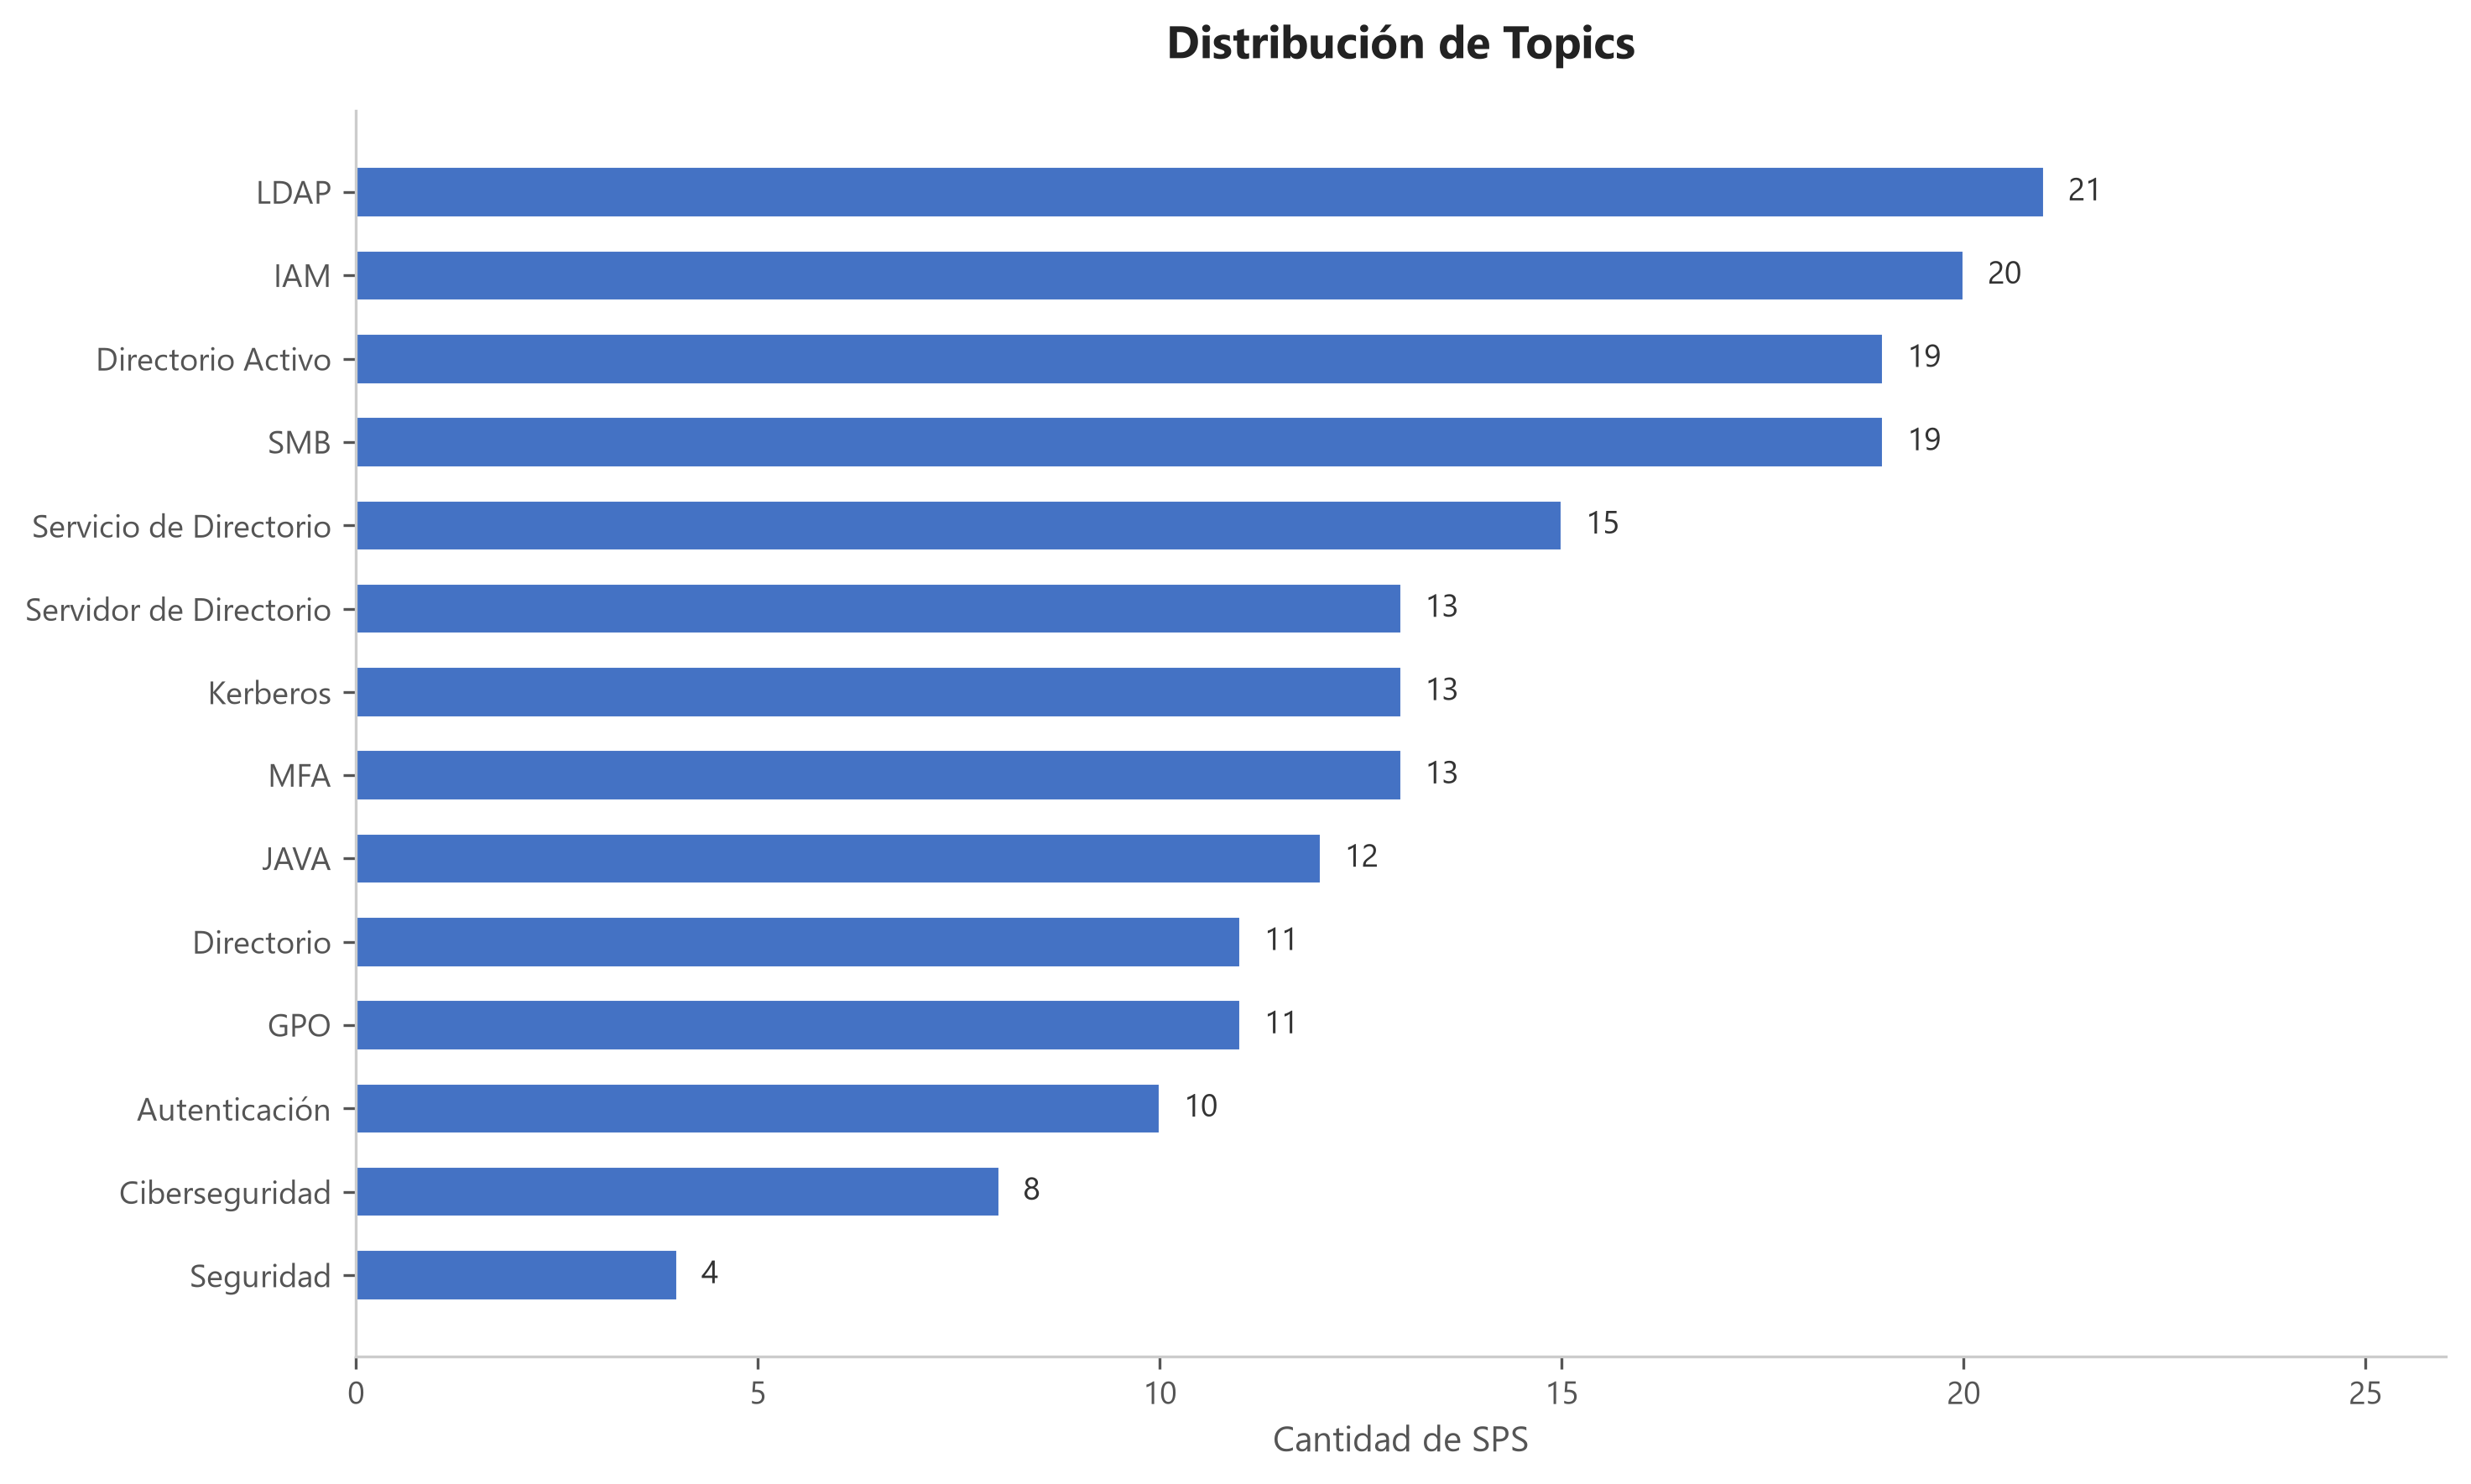
\includegraphics[width=0.9\textwidth]{mainmatter/II-desarrollo-metodologico/sms/imagenes/grafica-topicos.png}
	\caption{Diagrama de la distribución de los tópicos}
	\label{fig:grafica-topicos}
\end{figure}
